% Chapter 2

\chapter{Modelling the Ringdown from Precessing Black-hole Binaries}
\label{Chapter2}

\section{Introduction}
\label{ch2:sec:introduction}

In 2019 Giesler et al.~\cite{Giesler:2019uxc} demonstrated that using QNMs with $n > 0$ (that is, ringdown ``overtones'') could push the validity of the linear ringdown model to times as early as the peak of the GW strain. 
Their work involved fitting ringdown models to a selection of aligned-spin SXS simulations, and in this chapter we extend their work to misaligned-spin (i.e.\ precessing) systems.

The 2019 study sparked many other papers which involve fitting ringdown models with overtones to NR simulations~\cite{Bhagwat:2019dtm, Ota:2019bzl, JimenezForteza:2020cve, Cook:2020otn, Dhani:2020nik, Mourier:2020mwa, Dhani:2021vac, Forteza:2021wfq, MaganaZertuche:2021syq} (including the present work), but it should be noted that fears of over-fitting and the physical validity of the overtones were also present.
Even at the time of writing there is not a consensus on this point~\cite{Baibhav:2023clw, Nee:2023osy}, a central issue being that of the ringdown start time.

A prerequisite for any ringdown analysis is a suitable choice for the start time, $t_0$, of the ringdown. 
Starting too early risks obtaining biased measurements, because a GW signal contaminated with nonlinearities from the merger cannot be described by a model based solely on QNMs.
On the other hand, due to the exponential decay of the ringdown, starting too late leaves too little SNR to make useful measurements. 
In ringdown studies, typically the start time is given in reference to the maxima of some time-dependent quantity.
This could be the modulus of the $(2,2)$ mode of the strain or the $\Psi_4$ Weyl scalar, or the total GW luminosity; these quantities peak at times that typically differ by a few tens of $M$ (see Ref.~\cite{Berti:2007fi} for a discussion of some possible choices for the ringdown start time).
Often, to avoid concerns of fitting to the nonlinear merger, the ringdown start time is chosen to be $10M$ to $20M$ after the peak of these reference quantities. 
The work of Giesler et al.~\cite{Giesler:2019uxc}, which itself builds on previous studies of fitting ringdown models to NR simulations~\cite{Dorband:2006gg, Buonanno:2006ui, Berti:2007fi, Kamaretsos:2011um, Kamaretsos:2012bs, London:2014cma, Baibhav:2017jhs}, found that by including up to seven overtones the ringdown analysis can be started as early as the peak of the $(2,2)$ mode strain. 
This might be considered a surprising result; the signal peak is expected to occur when the remnant BH (to the extent that it yet even makes sense to consider it as such) is most highly distorted and linear perturbation theory is not expected to be valid. 
The failure of this intuition was investigated in Ref.~\cite{Okounkova:2020vwu} which suggests much of the nonlinearity is trapped behind a forming common apparent horizon and never makes it out to future null infinity in the form of GWs. 
Further support came from a study on the overtone excitation factors~\cite{Oshita:2021iyn}, which quantify the ease of excitation of the modes, and it was found that higher overtones are relatively easy to excite.
Even more surprising, Dhani~\cite{Dhani:2020nik} extended this approach via the inclusion of mirror modes along with overtones (thereby doubling the number of QNMs) and it was found that it was possible to start the ringdown analysis even earlier (up to $10M$ before the peak). 
Clearly it is not surprising that a model with so many free parameters is able to fit the GW signal well; the important point is that it is able to do so without obtaining biased values for the final mass and spin. 

The previous studies mentioned have only considered aligned-spin BBH systems, although we note that Ref.~\cite{Kamaretsos:2012bs} performed some limited analyses on precessing simulations.
We also note that some work on precessing systems has been done in the extreme mass ratio limit, see Refs.~\cite{Hughes:2019zmt,Lim:2019xrb,Lim:2022veo}.
It is well known that misalignment between the orbital angular momentum and the spins of the component BHs cause the orbit to precess during the inspiral phase of the evolution, leading to qualitatively different GW signals at early times (see, e.g., Ref.~\cite{Apostolatos:1994mx}). 
It is less clear what effect, if any, misaligned component spins would have on the late time ringdown signal which is generally associated with the remnant BH. 
The primary aim of this chapter is to address this question by systematically extending the analyses of Refs.~\cite{Giesler:2019uxc, Dhani:2020nik} to a large number of precessing BBH simulations from the SXS catalog~\cite{Boyle:2019kee}. 
We find that for BBH systems with misaligned spins, and that exhibit precession during their inspiral phase, a model consisting only of overtones (with or without mirror modes) cannot be reliably applied from the peak amplitude of the $(2,2)$ strain. 
A more conservative ringdown start time corresponding to the peak of the energy flux improves reliability, but we still see significant variation in performance across different simulations. 
The introduction of a higher harmonic (QNMs with $\ell > 2$) to the overtone model helps to reduce this variation, hinting at the importance of mode mixing.

Previous studies have focused on using full NR simulations to test ringdown models. 
In this chapter we also briefly investigate the use of surrogates, which provide an opportunity to test models over a continuous parameter space. 
We find caution should be taken, particularly for surrogates of precessing systems, due to errors in the surrogate waveforms.

In Section~\ref{ch2:sec:model} we write down the most general form of the ringdown model which will be used throughout this chapter.
The method used to fit the ringdown model to the SXS simulations is then explained in Section~\ref{ch2:sec:fitting}.
In Section~\ref{aligned-spin-section} we reproduce some important results from Refs.~\cite{Giesler:2019uxc, Dhani:2020nik}, which are later compared with those for precessing systems in Section~\ref{misaligned-spin-section}. 
With precessing systems, it is necessary to perform a frame rotation to account for the fact that the spin of the remnant BH will not be aligned with the initial coordinate axes used to set up the simulation; the procedure for doing this is also discussed in Section~\ref{misaligned-spin-section}. 
In Section~\ref{surrogate-section} we comment on the use of NR surrogates to test ringdown models. 
Finally, concluding remarks are presented in Section~\ref{sec:discussion}. 
Throughout, we use units in which $G=c=1$.

\section{Model for the spherical modes}
\label{ch2:sec:model}

NR expands the GW strain in the basis of (spin-weighted) spherical harmonics
\begin{equation}\label{ch2:eq:spherical_expansion}
    h = \sum_{\ell = 2}^\infty \sum_{m = -\ell}^\ell h_{\ell m}(t) {}_{-2}Y_{\ell m}(\Omega),
\end{equation}
where $\Omega$ is used as shorthand for the angles $\theta$, $\phi$.
By convention, the NR frame is uniquely fixed by requiring that initially the two component BHs are located on the $x$-axis and the orbital angular momentum, $\vb*{L}$, points along the $z$-axis.
The $h_{\ell m}(t)$ coefficients are referred to as the spherical-harmonic modes of the GW signal.
The $\ell=\abs{m}=2$ modes are typically largest, while the remaining ``higher modes'' are generally subdominant.
The output of an NR simulation usually includes the first few modes (e.g.\ $\ell \leq 8$) with the asymptotic radial dependence scaled out.
The spherical-harmonic modes are defined with respect to a particular frame at infinity, chosen such that the centre-of-mass of the system is at rest at some initial time. 
Note, however, that this still leaves freedom to perform an overall rotation (as will become important when we discuss precessing systems).

At late times ($t \geq t_0$, where $t_0$ is to be determined), perturbation theory expands the GW strain in the basis of the (spin-weighted) spheroidal harmonics
\begin{equation}\label{ch2:eq:spheroidal_expansion}
    h = \sum_{\ell =2}^\infty \sum_{m = -\ell}^\ell \sum_{n = 0}^\infty \left[ C_{\ell m n} e^{-i \omega_{\ell m n} (t - t_0)} {}_{-2}S_{\ell m n}(\Omega) + C'_{\ell m n} e^{-i \omega'_{\ell m n} (t - t_0)} {}_{-2}S'_{\ell m n}(\Omega) \right].
\end{equation}
Here, $C_{\ell m n}$ are complex coefficients (containing an amplitude and a phase), $\omega_{\ell m n} = 2\pi f_{\ell m n} - i/\tau_{\ell m n}$ are the complex QNM frequencies (which are functions of the remnant BH mass $M_f$ and spin $\chi_f$), and ${}_{-2}S_{\ell m n}(\Omega) = {}_{-2}S_{\ell m}(\Omega; a\omega_{\ell m n})$ are the spheroidal harmonics.
The spheroidal harmonics are functions of the spheroidicity $\gamma = a\omega_{\ell m n}$, where $a = M_f \chi_f$ is the Kerr parameter.
The primes denote the mirror modes, which satisfy $\operatorname{Re}[\omega'_{\ell m n}] = 2\pi f'_{\ell m n} < 0$.
As discussed in Section~\ref{ch1:sec:bh_spectroscopy}, these mirror modes are related to the regular modes via $\omega'_{\ell m n} = -\omega^*_{\ell -m n}$.
The prime on the spheroidal harmonic enters in the spheroidicity: ${}_{-2}S'_{\ell m n}(\Omega) = {}_{-2}S_{\ell m}(\Omega; a\omega'_{\ell m n})$.

It is important to note that Eq.~\ref{ch2:eq:spheroidal_expansion} is valid in a frame in which the remnant BH is at rest, with its spin vector pointing along the positive $z$-direction (such a frame is unique up to an unimportant rotation about the $z$-axis).
This ringdown frame is only the same as the NR frame for aligned-spin BBH systems (it is possible that systems with large component spins in the negative $z$-direction will exhibit a ``spin flip'', where the final spin also points in the negative $z$-direction; in these cases the two frames will only differ by a sign).
For misaligned-spin systems the remnant spin can point in essentially any direction and the NR and ringdown frames are misaligned; in these instances, as explained in Section~\ref{misaligned-spin-section}, we need to rotate the frame of the NR simulation to bring it into the ringdown frame where we can then apply Eq.~\ref{ch2:eq:spheroidal_expansion}.
The ringdown frame will also be moving with respect to the NR frame as a result of the recoil, or kick, from the anisotropic emission of GWs near merger. 
The effects of the kick are neglected here; it is assumed that the NR and ringdown frames are related by a rotation.

Assuming that the remnant BH spin vector is aligned with the $z$-axis in the NR frame (that is, the required rotation has been applied to the NR spherical-harmonic modes), we can equate Eqs.~\ref{ch2:eq:spherical_expansion} and \ref{ch2:eq:spheroidal_expansion} to get
\begin{equation}
    \sum_{\ell m} h_{\ell m}(t) {}_{-2}Y_{\ell m}(\Omega) = \sum_{\ell m n} \left[ C_{\ell m n} e^{-i \omega_{\ell m n} t} {}_{-2}S_{\ell m n}(\Omega) + C'_{\ell m n} e^{-i \omega'_{\ell m n} t} {}_{-2}S'_{\ell m n}(\Omega) \right],
\end{equation}
where we have dropped the limits on the sums for clarity.
We can then extract $h_{\ell m}$ using spherical-harmonic orthogonality:
\begin{align}\label{eq:hlm_with_ints}
    h_{\ell' m'}(t) = \sum_{\ell m n} \bigg[ &C_{\ell m n} e^{-i \omega_{\ell m n} t} \left(\int_\Omega \dd{\Omega} ~ {}_{-2}S_{\ell m n}(\Omega) ~ {}_{-2}Y^*_{\ell' m'}(\Omega)\right) \nonumber \\
    + &C'_{\ell m n} e^{-i \omega'_{\ell m n} t} \left(\int_\Omega \dd{\Omega} ~ {}_{-2}S'_{\ell m n}(\Omega) ~ {}_{-2}Y^*_{\ell' m'}(\Omega)\right) \bigg].
\end{align}
Following the convention of Ref.~\cite{Stein:2019mop}, the first integral is the spherical-spheroidal mixing coefficient:
\begin{equation}\label{ch2:eq:mu}
    \int_\Omega \dd{\Omega} ~ {}_{-2}S_{\ell m n}(\Omega) ~ {}_{-2}Y^*_{\ell' m'}(\Omega) = \mu_{\ell' m' \ell n} \delta_{m' m}.
\end{equation}
To evaluate the second integral we first rewrite the primed spheroidal harmonic as 
\begin{align}\label{eq:spheroidal_transform}
    {}_{-2}S'_{\ell m n}(\Omega) &= {}_{-2}S_{\ell m}(\theta, \phi; a\omega'_{\ell m n}) \nonumber \\
    &= {}_{-2}S_{\ell m}(\theta, \phi; -a\omega^*_{\ell -m n}) \nonumber \\
    &= (-1)^\ell {}_{-2}S^*_{\ell -m}(\pi - \theta, \phi; a\omega_{\ell -m n})
\end{align}
where the last line follows from Eqs.~48b and 48c of Ref.~\cite{Cook:2014cta}.
Next, we use the symmetries of the spherical harmonics to write
\begin{equation}\label{eq:spherical_transform}
    {}_{-2}Y^*_{\ell m}(\theta, \phi) = (-1)^{\ell} ~ {}_{-2}Y_{\ell -m}(\pi - \theta, \phi).
\end{equation}
Using Eqs.~\ref{eq:spheroidal_transform} and \ref{eq:spherical_transform} we can rewrite the second integral of Eq.~\ref{eq:hlm_with_ints} as
\begin{align}
    \int_\Omega \dd{\Omega}& ~ {}_{-2}S'_{\ell m n}(\Omega) ~ {}_{-2}Y^*_{\ell' m'}(\Omega) = \nonumber \\ 
    &= \int_\Omega \dd{\Omega} ~ (-1)^\ell {}_{-2}S^*_{\ell -m}(\pi - \theta, \phi; a\omega_{\ell -m n}) ~ (-1)^{\ell'} ~ {}_{-2}Y_{\ell' -m'}(\pi - \theta, \phi) \nonumber \\
    &= (-1)^{l+l'} \int_\Omega \dd{\Omega} ~ {}_{-2}S^*_{\ell -m}(\pi - \theta, \phi; a\omega_{\ell -m n}) ~ {}_{-2}Y_{\ell' -m'}(\pi - \theta, \phi) \nonumber \\
    &= (-1)^{l+l'} \mu^*_{\ell' -m' \ell n} \delta_{m' m}.
\end{align}
Substituting for both of the integrals of Eq.~\ref{eq:hlm_with_ints} we get
\begin{align}\label{ch2:eq:hlm_model}
    h_{\ell' m'}(t) &= \sum_{\ell m n} \left[ C_{\ell m n} e^{-i \omega_{\ell m n} t} \mu_{\ell' m' \ell n} \delta_{m' m} + C'_{\ell m n} e^{-i \omega'_{\ell m n} t} (-1)^{l+l'} \mu^*_{\ell' -m' \ell n} \delta_{m' m} \right] \nonumber \\
    &= \sum_{\ell n} \left[ C_{\ell m' n} e^{-i \omega_{\ell m' n} t} \mu_{\ell' m' \ell n} + C'_{\ell m' n} e^{-i \omega'_{\ell m' n} t} (-1)^{l+l'} \mu^*_{\ell' -m' \ell n} \right] \nonumber \\
    &= \sum_{\ell n} \left[ C_{\ell m' n} e^{-i \omega_{\ell m' n} t} \mu_{\ell' m' \ell n} + C'_{\ell m' n} e^{-i \omega'_{\ell m' n} t} \mu'_{\ell' m' \ell n} \right],
\end{align}
where $\mu'_{\ell' m' \ell n} = (-1)^{l+l'} \mu^*_{\ell' -m' \ell n}$.
Eq.~\ref{ch2:eq:hlm_model} tells us how a given spherical-harmonic mode (as provided by NR simulations) can be expressed in terms of QNMs. 
It reveals that each spherical-harmonic mode has contributions from every QNM of the same $m$, weighted by the spherical-spheroidal mixing coefficients; this is an effect known as mode mixing~\cite{Berti:2014fga}.

\section{Fitting implementation}
\label{ch2:sec:fitting}

Given some spherical-harmonic modes $h_{\ell m}$, we can turn Eq.~\ref{ch2:eq:hlm_model} into a least-squares fitting problem to find the best-fit complex coefficients $C_{\ell m n}$ and $C'_{\ell m n}$ (this assumes the complex frequencies and mixing coefficients are also given). 
First, we write Eq.~\ref{ch2:eq:hlm_model} as a matrix equation. 
Note that in the above we have separated the regular and mirror modes to show explicitly how to deal with the mirror modes (i.e. how to obtain their frequencies and mixing coefficients from the regular frequencies and mixing coefficients). 
We will now drop this distinction for clarity.

\subsection{Single-mode fit}

For simplicity, first consider the case when we want to model a single spherical mode (for example, the $h_{22}$ mode). We write
\begin{equation}\label{eq:hlm_matrix_single}
    \vb*{h}_{\ell m} = \vb*{a}_{\ell m} \vdot \vb*{C},
\end{equation}
where $\vb*{h}_{\ell m} = \qty(h_{\ell m}(t_0),\ h_{\ell m}(t_1),\ \ldots,\ h_{\ell m}(t_{K-1}))$ is the waveform data discretely sampled at a total of $K$ times labelled by $t_k$. 
In general $t_0$ may not exist on the default array of simulation times, so care must be taken (for example, we can interpolate the simulation data and evaluate on a new grid of times, or we could use the first value after $t_0$, or the closest value to $t_0$). 

The matrix $\vb*{a}_{\ell m}$ is where the choice of QNM content in our model enters. 
It has the form
\begin{equation}
    \vb*{a}_{\ell m} = 
    \begin{pmatrix}
    e^{-i \omega_0 (t_0 - t_0)} \mu_{\ell m,0} & e^{-i \omega_1 (t_0 - t_0)} \mu_{\ell m,1} & \cdots & e^{-i \omega_{J-1} (t_0 - t_0)} \mu_{\ell m,J-1} \\ 
    e^{-i \omega_0 (t_1 - t_0)} \mu_{\ell m,0} & e^{-i \omega_1 (t_1 - t_0)} \mu_{\ell m,1} & \cdots & e^{-i \omega_{J-1} (t_1 - t_0)} \mu_{\ell m,J-1} \\ 
    \vdots & \vdots & \ddots & \vdots \\
    e^{-i \omega_0 (t_{K-1} - t_0)} \mu_{\ell m,0} & e^{-i \omega_1 (t_{K-1} - t_0)} \mu_{\ell m,1} & \cdots & e^{-i \omega_{J-1} (t_{K-1} - t_0)} \mu_{\ell m,J-1}
    \end{pmatrix},
\end{equation}
where we have suppressed the three QNM labels and instead labelled each QNM by a single number. 
There are a total of $J$ QNMs included in the model.
So, $\vb*{a}_{\ell m}$ is a matrix of shape $(K, J)$.
To reiterate, the QNM content in our model can consist of any regular or mirror modes, as long as the correct frequencies and mixing coefficients are used in the above matrix (we have just used $\omega_j$ and $\mu_{\ell m, j}$ as generic terms). 

The vector $\vb*{C}$ contains our complex amplitudes, of which there are a total of $J$ (one for each QNM included in the model). This has the form
\begin{equation}
    \vb*{C} = \left(C_0,\ C_1,\ \ldots,\ C_{J-1}\right)^T.
\end{equation}
When we perform the matrix multiplication of Eq.~\ref{eq:hlm_matrix_single} we are multiplying a matrix of shape $(K,J)$ by a vector of length $J$, so we are left with a vector of length $K$.
Written in this form, we can easily apply least-squares solvers to invert the equation for the vector of coefficients. 
This minimises the Euclidean 2-norm $\norm{\vb*{h}_{\ell m} - \vb*{a}_{\ell m} \vdot \vb*{C}}$ (i.e.\ the sum of the squares of the fit residuals).
In this chapter we will only be dealing with single-mode fits as described here.
However, for completeness, below we describe how multimode fits can be implemented (available in the code developed for this work~\cite{qnmfits}).

\subsection{Multimode fit}

Due to mode mixing, a given QNM contributes to all spherical-harmonic modes with the same $m$. 
This means we can perform a fit to multiple spherical-harmonic modes with a single set of shared QNM amplitudes $\vb*{C}$.
We will approach this by joining $\vb*{h}_{\ell m}$ vectors together for each $(\ell, m)$ we want to include in the fit (to effectively form a single time series), and similarly by ``stacking'' $\vb*{a}_{\ell m}$ matrices on top of each other.

The single-mode matrix equation, Eq.~\ref{eq:hlm_matrix_single}, becomes
\begin{equation}\label{eq:hlm_matrix_multi}
    \vb*{h} = \vb*{a} \vdot \vb*{C},
\end{equation}
where
\begin{equation}
    \vb*{h} = 
    \begin{bmatrix}
    \vb*{h}_0 & \vb*{h}_1 & \cdots & \vb*{h}_{I-1}
    \end{bmatrix}
\end{equation}
and $I$ is the number of spherical-harmonic modes to include in the fit (we have suppressed the two spherical-harmonic indices for clarity). So, $\vb*{h}$ is a vector of length $I \times K$.
Similarly
\begin{equation}
    \vb*{a} = 
    \begin{bmatrix}
    \vb*{a}_0 \\ \vb*{a}_1 \\ \vdots \\ \vb*{a}_{I-1}
    \end{bmatrix},
\end{equation}
which has shape $(I \times K, J)$. 
We see that when we multiply this new coefficient matrix by the vector $\vb*{C}$ (length $J$) in Eq.~\ref{eq:hlm_matrix_multi} we recover a vector of correct length $I \times K$.

The quantity we're minimising is now
\begin{equation}
    \norm{\vb*{h} - \vb*{a} \vdot \vb*{C}} = \sqrt{ \sum_{\ell m} \norm{\vb*{h}_{\ell m} - \vb*{a}_{\ell m} \vdot \vb*{C}}^2 }
\end{equation}
which gives equal ``weight'' to each $(\ell,m)$ mode, and can be shown to be equivalent as averaging the least-squares fit over the sky.

\section{Aligned-spin systems}\label{aligned-spin-section}

Following Giesler et al.~\cite{Giesler:2019uxc}, the spherical-harmonic modes of the ringdown signal can be modelled by writing each as a sum of $N$ overtones:
\begin{equation}\label{GieslerRD}
    h_{\ell m}^N(t) = \sum_{n=0}^N C_{\ell m n} e^{-i\omega_{\ell m n}(t-t_0)}, \quad \textrm{for} \quad t \geq t_0.
\end{equation}
This \emph{overtone} model is a restriction of the sum in Eq.~\ref{ch2:eq:hlm_model}, where overlaps between different harmonic $\ell$ indices (mode mixing) as well as mirror modes are neglected. 
As in Ref.~\cite{Giesler:2019uxc}, we model each spherical-harmonic mode individually as a sum of QNMs.
In Ref.~\cite{Giesler:2019uxc}, the efficacy of this model for $\ell=m=2$ was demonstrated by performing least squares fits to the $h_{22}$ mode for a selection of aligned-spin SXS simulations. The authors note that this was also verified for other values of $(\ell,m)$.

The overtone model in Eq.~\ref{GieslerRD} contains $2(N+1)$ free parameters in the complex amplitudes, $C_{\ell m n}$, plus the two parameters, $M_f$ and $\chi_f$, that determine the $\omega_{\ell m n}$ frequencies.
All of these parameters depend on the properties of the progenitor binary, but we do not study these dependencies here.

Our fitting algorithm finds the amplitudes $C_{\ell m n}$ that minimise the sum-of-the-squares of the fit residuals.
We find it convenient to treat the remnant property parameters $M_f$ and $\chi_f$ differently from the excitation amplitudes. 
If we also want to minimise over the remnant properties (as opposed to fixing them to the true values given by NR) then first a discrete 2-dimensional numerical grid of values for $M_f$ and $\chi_f$ is constructed.
At each point on this grid, we consider varying only the complex amplitudes $C_{\ell m n}$. 
Eq.~\ref{eq:hlm_matrix_single} turns this minimisation problem into a linear algebra problem that can be efficiently solved with, for example, \texttt{numpy.linalg.lstsq}~\cite{Harris:2020xlr}.
Finally, the point of the grid with the lowest overall value for the sum-of-the-squares of the fit residuals is chosen.

Once the least-squares fit to the data has been obtained, the quality of the fit is quantified via the mismatch and the error on the remnant parameters.
The mismatch between signals $h_1$ and $h_2$ is defined as
\begin{equation}\label{mismatch}
    \mathcal{M} = 1 - \frac{\Re[\braket{h_1}{h_2}]}{\sqrt{\braket{h_1}\braket{h_2}}},
\end{equation}
where we use the following complex inner product~\cite{Nollert:1998ys}
\begin{equation} \label{eq:inner_prod}
    \braket{h_1}{h_2} = \int_{t_0}^T h_1(t) h^*_2(t) ~ \dd t.
\end{equation}
We integrate from the ringdown start time, $t_0$, to an upper limit $T$ chosen such that the whole ringdown is captured (we use $T = t_0 + 100M$).
When fitting models with very small mismatches, the finite accuracy of the NR simulations must be considered; this is discussed in Section~\ref{NR_error_appendix}.
As noted in Ref.~\cite{Giesler:2019uxc}, a small mismatch is not sufficient by itself to justify the model.
The overtone model contains more parameters as $N$ is increased, and it is necessary to check for over-fitting.
To address this, we check to see if the remnant BH properties are correctly recovered by the model. 
The combined error on the remnant mass and spin is quantified by~\cite{Giesler:2019uxc}
\begin{equation} \label{eq:epsilon}
    \epsilon = \sqrt{ \left( \frac{\delta M_f}{M} \right)^2 + \left( \delta\chi_f \right)^2 },
\end{equation}
where $\delta M_f = M_{\mathrm{best fit}} - M_f$, and $\delta \chi_f = \chi_{\mathrm{best fit}} - \chi_f$. 
The best fit values are those which minimise the mismatch, while the true values are taken from the metadata for the SXS simulation.
A ringdown model can be said to perform well if it yields small values for both $\mathcal{M}$ and $\epsilon$.

\begin{figure}[t]
    \centering
    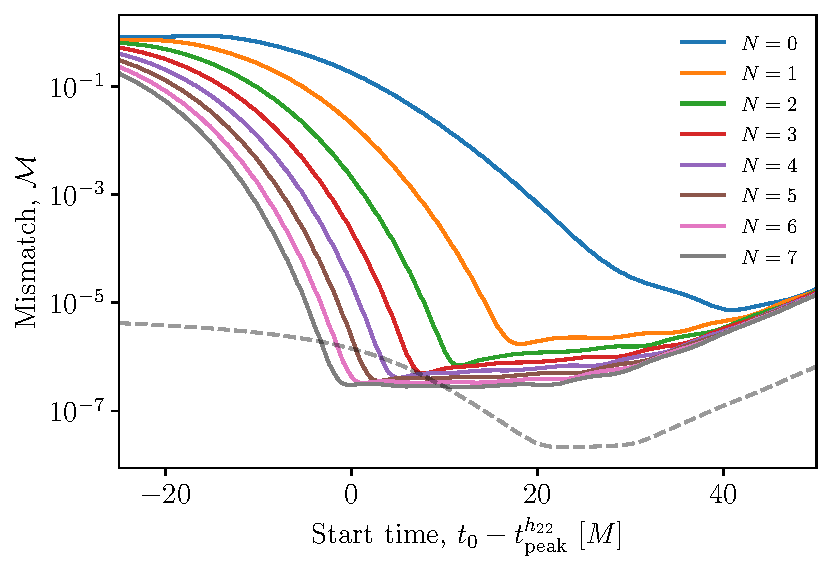
\includegraphics[width=0.6\columnwidth]{ModellingTheRingdownFromPrecessingBlackHoleBinaries/305_mismatch_vs_t0_with_error.pdf}
    \caption[Mismatch of the overtone model fitted to SXS:BBH:0305]{ 
    Mismatch as a function of ringdown start time for the overtone model (Eq.~\ref{GieslerRD}) when fitting to the $h_{22}$ mode of the NR simulation SXS:BBH:0305. 
    When using only the fundamental $\ell = m = 2$, $n = 0$ QNM the start time that gives the lowest mismatch with the NR data is well after the merger (the rising mismatch at late times is a numerical artefact). 
    However, reproducing the results from Ref.~\cite{Giesler:2019uxc}, we find that by including $N=7$ overtones the GW signal can be fitted using QNMs starting from as early as the peak strain. 
    The dashed grey curve shows the estimate of the error in the underlying NR simulation and is described in Section~\ref{NR_error_appendix}.
    }
    \label{305_mismatch_vs_t0}
\end{figure}

\begin{figure}[t]
    \centering
    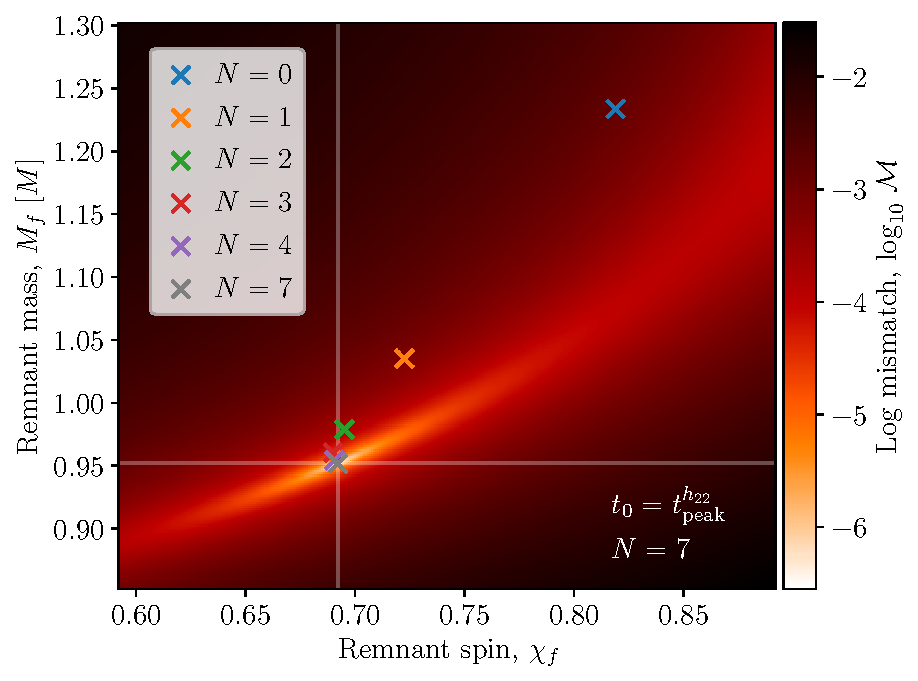
\includegraphics[width=0.6\columnwidth]{ModellingTheRingdownFromPrecessingBlackHoleBinaries/305_epsilon_grid.pdf}
    \caption[Recovery of SXS:BBH:0305 remnant properties using the overtone model]{ 
    Recovery of the SXS:BBH:0305 remnant properties when fitting the overtone model (Eq.~\ref{GieslerRD}) to the $h_{22}$ mode from the time of its peak strain.
    The heat map shows the mismatch for the fit with $N=7$ overtones, which shows a pronounced minimum close ($\epsilon=3.4\times 10^{-4}$) to the true remnant parameters (indicated by the horizontal and vertical lines).
    The sequence of crosses shows the locations of the minima for fits performed with different values of $N$, all using the same start time (the cross colours correspond to the colours used in Fig.~\ref{305_mismatch_vs_t0}; crosses for $N=5$ and 6 are omitted to avoid crowding the plot, but they converge towards the true remnant parameters). 
    If we choose a different ringdown start time for each $N$ corresponding to the mismatch minima in Fig.~\ref{305_mismatch_vs_t0}, we do see a reduction in $\epsilon$ for the lower $N$ models, however the $N=7$ model with $t_0=t_\mathrm{peak}^{h_{22}}$ remains the best performing model.
    } 
    \label{305_epsilon_grid}
\end{figure}

Following Ref.~\cite{Giesler:2019uxc}, we now apply these ideas to the simulation SXS:BBH:0305~\cite{Lovelace:2016uwp}.
This simulation has source parameters consistent with GW150914 and was originally chosen to demonstrate the success of the overtone model. 
Fig.~\ref{305_mismatch_vs_t0} shows the mismatch values obtained with the overtone model when using the true values of $M_f$ and $\chi_f$.
With $N=7$ (that is, eight QNMs = the fundamental mode + seven overtones) the $h_{22}$ mode can be fitted all the way back to the time of its peak amplitude, $t_{\mathrm{peak}}^{h_{22}}$, while still achieving the smallest possible mismatch.
Using a smaller number of overtones requires a later choice for the start time to achieve the smallest possible mismatch.
In addition to giving a small ($\sim 10^{-6}$) mismatch, the $N=7$ overtone model, with $t_0 = t_{\mathrm{peak}}^{h_{22}}$, also achieves this minimum mismatch with the correct values for the remnant properties; this is shown by the heat map in Fig.~\ref{305_epsilon_grid} where the values of $M_f$ and $\chi_f$ are now allowed to vary. 
We find, for the $N=7$ model, a remnant error $\epsilon = 3.4 \cross 10^{-4}$. 
Importantly, this is larger than the NR error on the remnant properties (which is estimated to be $\epsilon_{\mathrm{NR}} = 2.1 \cross 10^{-5}$, see Section~\ref{NR_error_appendix} for details). This confirms that this is really the true scale of the bias in the inferred remnant parameters when using the overtone model, and not just the numerical noise floor in the NR simulation.
Again, using a smaller number of overtones and starting the ringdown as early as $t_{\mathrm{peak}}^{h_{22}}$ gives inferior results with the minimum in the mismatch being biased away from the true parameters.
The results in Figs.~\ref{305_mismatch_vs_t0} and \ref{305_epsilon_grid} show that the overtone model performs well for SXS:BBH:0305 (i.e.\ yields small $\mathcal{M}$ and $\epsilon$) even when starting the ringdown as early as the peak in the strain.

\begin{figure}[t]
    \centering
    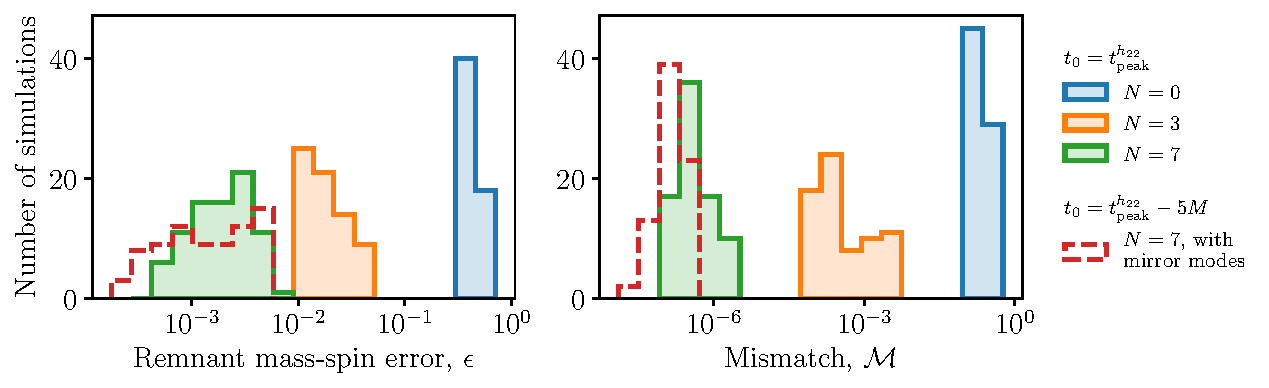
\includegraphics[width=\columnwidth]{ModellingTheRingdownFromPrecessingBlackHoleBinaries/aligned_spin_epsilon_M_hist.pdf}
    \caption[Remnant-property errors and mismatches for the overtone model fitted to aligned-spin SXS simulations]{\emph{Left:} histograms of the mass-spin remnant error $\epsilon$ from an overtone-model fit to 85 aligned-spin SXS simulations for several different overtone numbers $N$. 
    \emph{Right:} histograms of the mismatch from a fit with the true remnant mass and spin parameters, with the same overtone models and SXS simulations as in the left histogram.
    The solid histograms show results from fits performed starting at the peak of the $h_{22}$ mode with $N$ overtones of the fundamental $\ell = m = 2$ mode.
    The red dashed line shows results from a $N=7$ model that also includes mirror modes (see Section~\ref{subsec:mirror_modes}) and was fitted with a ringdown starting $5M$ before the peak of the strain.}
    \label{aligned_spin_epsilon_hist}
\end{figure}

In order to see how robust the conclusions drawn from SXS:BBH:0305 are in general, the calculations of $\epsilon$ and $\mathcal{M}$ were repeated for a wider selection of SXS simulations. Following Ref.~\cite{Giesler:2019uxc}, we consider only aligned-spin simulations with initial spin magnitudes $|\vb*{\chi}_{1,2}| = \chi_{1,2} < 0.8$, and mass ratios $q < 8$. We also require that the $z$-component of $\vb*{\chi}_f$ is greater than zero, which eliminates the ``spin flip'' systems. The simulations were chosen in the ID range SXS:BBH:1412 to SXS:BBH:1513, as these cover a range of initial spin magnitudes and mass ratios.
After applying these cuts, this left 85 spin-aligned SXS simulations in our test set.
For each simulation, fits were performed using the overtone model with $N=0$, 3, and 7 and with a start time of $t_0 = t_{\mathrm{peak}}^{h_{22}}$. 
The results are shown in Fig.~\ref{aligned_spin_epsilon_hist}. 
We see distributions similar to those in Fig.~3 of Ref.~\cite{Giesler:2019uxc}. 
The inclusion of additional overtones systematically shifts the entirety of both the $\epsilon$ and $\mathcal{M}$ histograms to smaller values.
We note, as it will become important later, that the worst cases in these histograms improve, along with the median values.
This demonstrates that, when using the overtone model on systems with aligned spins, the ringdown reliably starts as early as the peak in the $h_{22}$ mode of the strain. 


\subsection{Mirror modes} \label{subsec:mirror_modes}

For a given $\ell$, $m$ and $n$, the equations governing QNM frequencies allow two solutions: one, $\omega_{\ell m n} = 2\pi f_{\ell m n} - i/\tau_{\ell m n}$, with a positive real part; and another, $\omega'_{\ell m n} = 2\pi f'_{\ell m n} - i/ \tau'_{\ell m n}$, with negative real part~\cite{Dhani:2020nik, Berti:2005ys}.
The frequencies of the mirror modes $\omega'_{\ell m n}$ are related to the regular modes $\omega_{\ell m n}$ by Eq.~\ref{ch1:eq:mirror}.

A new ringdown model which explicitly includes the mirror modes can be written as
\begin{equation}
    h_{\ell m}^{N,\, {\rm mirror}}(t) = \sum_{n=0}^N \qty[ C_{\ell m n} e^{-i \omega_{\ell m n}(t-t_0)} + C'_{\ell m n} e^{-i \omega'_{\ell m n}(t-t_0)} ]\quad \textrm{for} \quad t \geq t_0.
\end{equation}
This \emph{mirror-mode} model is an extension of the overtone model in Eq.~\ref{GieslerRD}; if $C'_{\ell m n} = 0$ the mirror modes aren't excited and we recover the previous overtone model. 
This model has twice as many free parameters as the overtone model; $4(N+1)$ in the complex amplitudes, plus the two remnant parameters $M_f,\; \chi_f$.
The mirror-mode model is still a restriction of the full sum in Eq.~\ref{ch2:eq:hlm_model} as overlaps between modes with different $\ell$ indices (i.e.\ mode mixing) are still not included.
Substituting for $\omega'_{\ell m n}$ using the conjugate symmetry property in Eq.~\ref{ch1:eq:mirror}, we can rewrite the mirror-mode model in the form
\begin{equation} \label{ch2:eq:mirror_model}
   h_{\ell m}^{N,\, {\rm mirror}}(t) = \sum_{n=0}^N \qty[ C_{\ell m n} e^{-i \omega_{\ell m n}(t-t_0)} + C'_{\ell m n} e^{i \omega^*_{\ell -m n}(t-t_0)} ]\quad \textrm{for} \quad t \geq t_0.
\end{equation}
This is how the model was implemented in practice.

As was shown by Dhani~\cite{Dhani:2020nik}, the inclusion of mirror modes can improve the ringdown modelling of aligned-spin systems. In particular, the ringdown can be considered to start even earlier in the waveform, whilst still recovering the correct remnant properties. We confirm this here by repeating the above analysis for the same set of spin-aligned SXS simulation, but now using the mirror-mode model in Eq.~\ref{ch2:eq:mirror_model} with $N=7$ and an earlier choice for the ringdown start time, $t_0 = t_{\mathrm{peak}}^{h_{22}} - 5M$.
Although Ref.~\cite{Dhani:2020nik} demonstrated the mirror-mode model starting $10M$ before the peak in the $h_{22}$ strain, we adopt a more conservative choice of $5M$.
The results are shown in Fig.~\ref{aligned_spin_epsilon_hist} using a dashed line. 
The addition of mirror modes gives a small improvement in the mismatch, but this is to be expected with the increased number of parameters.
However, the $\epsilon$ histogram shows that the overall performance of the mirror-mode model is comparable to that of the $N=7$ overtone model, despite the use of an earlier start time.


\section{Misaligned-spin systems}\label{misaligned-spin-section}

The analyses in Section~\ref{aligned-spin-section}, and analyses in previous studies,
% ~\cite{Dorband:2006gg, Buonanno:2006ui, Berti:2007fi, Kamaretsos:2011um, Kamaretsos:2012bs, London:2014cma, Baibhav:2017jhs, Giesler:2019uxc, Bhagwat:2019dtm, Ota:2019bzl, JimenezForteza:2020cve, Cook:2020otn, Dhani:2020nik, Mourier:2020mwa, Forteza:2021wfq, MaganaZertuche:2021syq},
was limited to BBH systems with component spins that are aligned with the orbital angular momentum, $\vb*{L}$.
This is a potentially serious limitation as misaligned spins are expected to be a generic feature of astrophysical BBHs.
Misaligned spins generally lead to precession of the orbital plane during the inspiral phase of the evolution and a richer phenomenology in the GW signals~\cite{Apostolatos:1994mx}.
There is strong evidence for precession in the GW events observed so far when looking at the population level~\cite{LIGOScientific:2020kqk, LIGOScientific:2021psn}, and tentative evidence in individual events. 
This includes high-mass event GW190521~\cite{LIGOScientific:2020iuh, LIGOScientific:2020ufj}, the asymmetric-mass event GW190412~\cite{LIGOScientific:2020stg}, and recently there have been claims of precession in the GWTC-3 event GW200129\_065458~\cite{Hannam:2021pit} (but we note that there are potential data-quality issues associated with this event~\cite{Payne:2022spz}).
In this section we investigate the effect of precession on the modelling of the ringdown by repeating analyses like those in Section~\ref{aligned-spin-section}, but now on precessing NR simulations.

As already mentioned, the remnant BH will not have a spin vector aligned with the $z$-axis in the NR frame if it has undergone precession. 
The ringdown models we have been using are only valid in the frame with the remnant BH spin vector aligned with the $z$-axis.
Therefore, before applying the ringdown models to precessing NR data, we need to rotate the NR data into the suitable frame. 

The direction from which a GW source is viewed affects the observed signal 
(e.g.\ you see circularly/linearly polarised GWs with a larger/smaller amplitude when viewing parallel/perpendicular to $\vb*{L}$).
These differences in the GW signals also manifest themselves at the level of individual spherical-harmonic modes as amplitude modulations. 
The frame in which the expansion (Eq.~\ref{ch2:eq:spherical_expansion}) is performed affects the values of the spherical-harmonic modes. 
The idea is to re-expand the NR data in the ``ringdown frame'' as follows:
\begin{equation}\label{hprimedecomp}
    h' = \sum_{\ell = 2}^\infty \sum_{m = -\ell}^\ell h'_{\ell m}(t) {}_{-2}Y_{\ell m}(\Omega'),
\end{equation}
where the prime on $\Omega$ indicates we are using new coordinates where the remnant spin is aligned with the $z$-axis.
The coefficients in this expansion, $h'_{\ell m}$, are what we now fit our ringdown models to. 
In particular, we will focus on modelling the $\ell = m = 2$ spherical harmonic mode in the ringdown frame, $h'_{22}$.

For aligned-spin systems, the $h_{2\pm2}$ are usually the dominant modes in the sum in Eq.~\ref{ch2:eq:spherical_expansion}. This is related to the fact that the GW signal amplitude is largest when viewed along the direction of the orbital angular momentum: $\vb*{L}$ or $-\vb*{L}$. For misaligned-spin systems undergoing precession, other modes become important. This in turn is related to the constantly changing direction of the orbital angular momentum, $\vb*{L}(t)$.
Changing into the non-inertial, coprecessing frame in which $\vb*{L}$ always points along the $z$-direction has been found to account for most precessional effects and makes the precessing waveform remarkably similar to a non-precessing one.
This transformation into the coprecessing frame has been successfully used to help model the full inspiral-merger-ringdown waveforms for precessing systems~\cite{Schmidt:2010it, Schmidt:2012rh} in the context of phenomenological~\cite{Hannam:2013oca, Khan:2018fmp, Pratten:2020ceb}, effective-one-body~\cite{Pan:2013rra, Ossokine:2020kjp} and NR surrogate~\cite{Blackman:2017dfb, Blackman:2017pcm, Varma:2019csw} modelling.
There is an analogy with the approach taken here for the modelling of the ringdown. In order to simplify the task, we choose to work in a frame adapted to final spin angular momentum of the remnant, $\vb*{\chi}_f$.
Although, in our case, the rotation required to get into this frame is not time dependent and our chosen frame is therefore inertial.

The spin-weighted spherical harmonics, ${}_{-2}Y_{\ell m}$, transform in a particularly simple manner under rotations.
Rotations have the effect of mixing together modes with different $m$ indices, but preserving the same $\ell$. 
The mixing coefficients for a rotation $\mathbf{R}$ are the Wigner $D$-matrices $D^{\ell}_{\mu m} (\mathbf{R})$.
The transformation properties of the ${}_{-2}Y_{\ell m}$ functions under rotations means that the rotated $h'_{\ell m}$ modes in the ringdown frame are related to the $h_{\ell m}$ modes in the NR frame (included in the NR output, and as used in Section~\ref{aligned-spin-section}) by the sum (see, for example, Refs.~\cite{Boyle:2013nka, Schmidt:2010it, OShaughnessy:2011pmr})
\begin{align}\label{Yrotation_wignerD}
    h'_{\ell m}(t) &= \sum_{\mu = -\ell}^{\ell} D^{\ell}_{\mu m} (\mathbf{R}) ~ h_{\ell \mu}(t).
\end{align}
The rotation $\mathbf{R}$ can be obtained from the direction of the remnant BH spin vector (which is provided as metadata for all SXS simulations). Specifically, $\mathbf{R}$ is any rotation that maps the $z$-axis onto the final spin vector.

We now apply the overtone model to the ringdown of an example precessing simulation SXS:BBH:1856~\cite{Varma:2019csw}. 
This simulation (at the reference time) has a mass ratio of $q=2.78$ and dimensionless spins $\vb*{\chi}_1=(0.18, -0.54, -0.45)$ and $\vb*{\chi}_2=(-0.12, -0.31, -0.031)$ on the heavier and lighter components respectively. 
This simulation was chosen because it exhibits strong precession effects visible as amplitude modulations in $h_{22}(t)$. The final spin vector is $\vb*{\chi}_f=(-0.03,-0.19,0.42)$ and the rotated mode $h'_{22}(t)$ was computed using Eq.~\ref{Yrotation_wignerD}.

\begin{figure}[t]
    \centering
    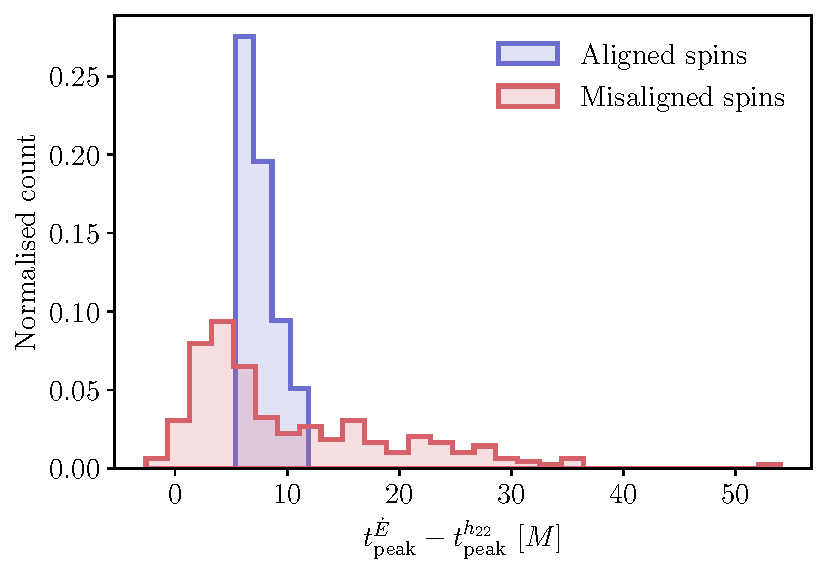
\includegraphics[width=0.6\columnwidth]{ModellingTheRingdownFromPrecessingBlackHoleBinaries/tEdot-t22_hist.pdf}
    \caption[Differences in the times of peak strain amplitude and peak luminosity]{  
    Histogram of the differences between the two possible start times considered in Section~\ref{misaligned-spin-section}: the peak of the (rotated) strain mode $h'_{22}$, and the peak of the GW energy flux.
    The normalised distribution of the differences between these times is shown both for the 85 spin-aligned systems used in Section~\ref{aligned-spin-section} and for the 252 precessing simulations considered in Section~\ref{misaligned-spin-section}. 
    The peak of the flux almost always occurs later than the peak of the strain, making this a more conservative choice for the ringdown start time. 
    We note that there is a much greater variation amongst the population with misaligned spins.
    }
    \label{tEdot-t22}
\end{figure}

The overtone model in Eq.~\ref{GieslerRD} was fitted to the rotated $\ell=m=2$ mode of the strain, $h'_{22}(t)$, in the same way as was done for the aligned-spin systems in Section~\ref{aligned-spin-section}.
There is some ambiguity in how to choose the ringdown start time $t_0$ in a way that gives as fair a comparison as possible with the non-precessing case. 
We cannot use the peak of the $h_{22}(t)$ strain, as was done in Section~\ref{aligned-spin-section}, as this mode suffers from precession induced amplitude modulations. 
One option would be to use instead the peak of the rotated strain mode $h'_{22}(t)$.
However, we find that using the peak of the GW energy flux, $\dot{E}$, (which can be computed from the modes in either frame, see Eq.~3.8 in Ref.~\cite{Ruiz:2007yx}) gives more consistent results between simulations. For example, some precessing configurations show a peak in the (rotated) strain relatively early in the signal, leading to poorer fits.
The use of the peak in the energy flux is also a conservative choice in the sense that $t_{\mathrm{peak}}^{\dot{E}} > t_{\mathrm{peak}}^{h_{22}}$ in almost all cases (see Fig.~\ref{tEdot-t22}).

\begin{figure}[t]
    \centering
    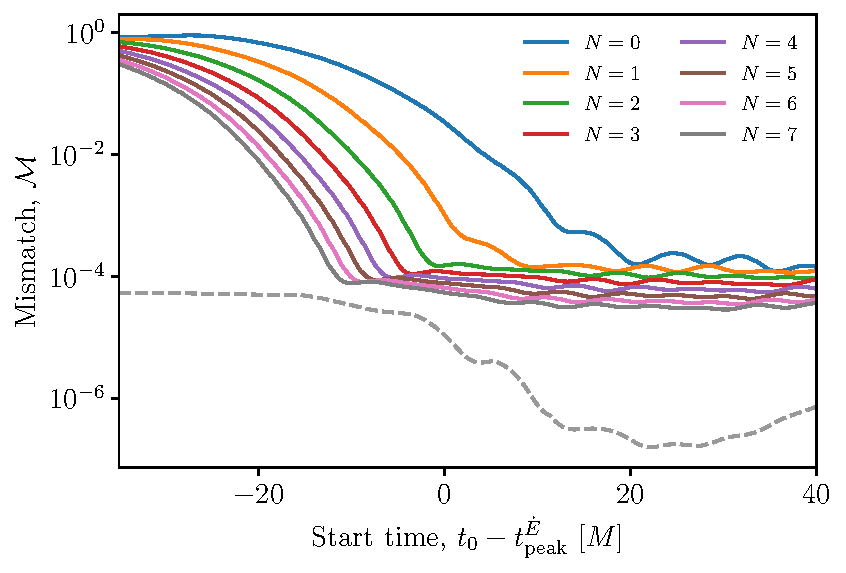
\includegraphics[width=0.6\columnwidth]{ModellingTheRingdownFromPrecessingBlackHoleBinaries/1856_mismatch_vs_t0_with_error_edit.pdf}
    \caption[Mismatch for the overtone model fitted to SXS:BBH:1856]{
    Mismatch as a function of ringdown start time for the overtone model (Eq.~\ref{GieslerRD}) when fitting to the rotated $h'_{22}$ mode of the NR simulation SXS:BBH:1856.
    When using $N=7$ overtones, the lowest mismatch is achieved starting slightly ($\sim 10M$) before the peak in the GW energy flux.
    However, the minimum mismatch is $\sim 100$ times larger than that obtained for the example spin-aligned system SXS:BBH:0305 in Fig.~\ref{305_mismatch_vs_t0}. 
    The dashed grey curve shows the estimate of the error in the underlying NR simulation and is described in Section~\ref{NR_error_appendix}.
    }
    \label{1856_mismatch_vs_t0}
\end{figure}

Fig.~\ref{1856_mismatch_vs_t0} shows how the mismatch varies for SXS:BBH:1856 as a function of ringdown start time, for different values of $N$ in the overtone model Eq.~\ref{GieslerRD}.
With each additional overtone, the minimum mismatch is reached at an earlier time (the same behaviour as was seen in Fig.~\ref{305_mismatch_vs_t0}).
However, the values of the minimum mismatch are a factor of $\sim 100$ larger than those obtained in the aligned-spin case. 

The $N=7$ model achieves a minimum mismatch $\sim 10M$ before the time of peak GW energy flux. This is fairly typical behaviour among the misaligned-spin SXS simulations considered.
However, we note there is a much greater variety of possible behaviours for misaligned-spin systems than for the aligned-spin population. 
The greater variation amongst the misaligned-spin population has already been hinted at in Fig.~\ref{tEdot-t22}, where the spread of start times is greater than in the aligned-spin cases.

\begin{figure}[t]
    \centering
    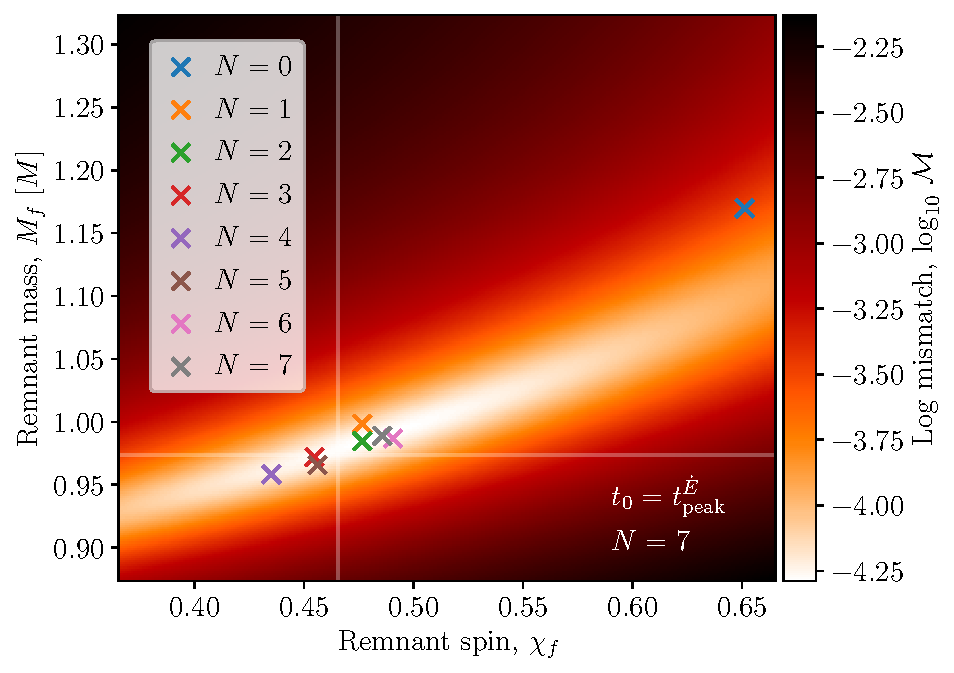
\includegraphics[width=0.6\columnwidth]{ModellingTheRingdownFromPrecessingBlackHoleBinaries/1856_epsilon_grid_alt.pdf}
    \caption[Recovery of SXS:BBH:1856 remnant properties using the overtone model]{
    Recovery of the SXS:BBH:1856 remnant properties when fitting the overtone model (Eq.~\ref{GieslerRD}) to the rotated $h'_{22}$ mode from the time of its peak energy flux.
    The heat map shows the mismatch for the fit with $N=7$, while the crosses show the locations of the minima in the mismatch for fits performed with different values of $N$.
    The mismatch shows a much broader and less deep minimum than that seen for the spin-aligned system SXS:BBH:0305 in Fig.~\ref{305_epsilon_grid}.
    The minimum in the mismatch is also biased away from the true remnant parameters with $\epsilon=0.025$ for the $N=7$ fit.
    The sequence of crosses for fits with different values of $N$ also do not show the same convergent trend towards the true remnant parameters that was observed for SXS:BBH:0305 in Fig.~\ref{305_epsilon_grid}.
    }
    \label{1856_epsilon_grid}
\end{figure}

\begin{figure}[t]
    \centering
    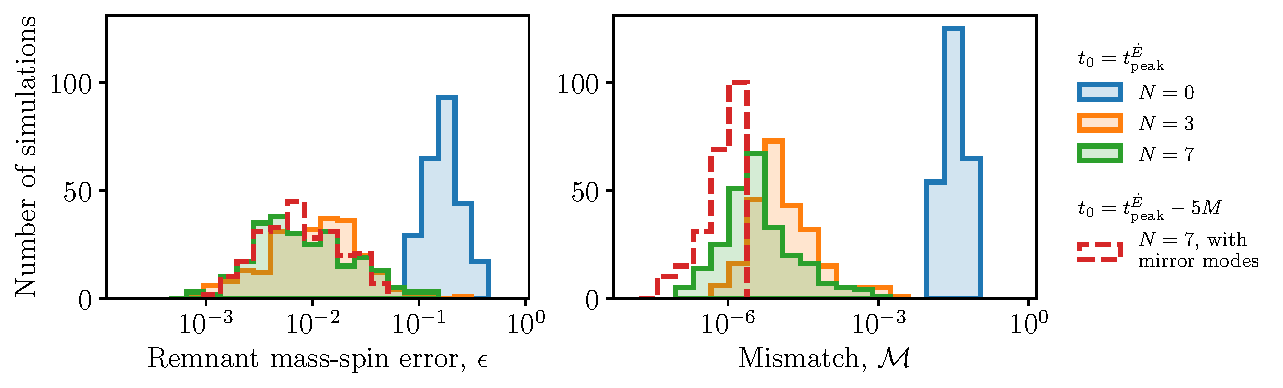
\includegraphics[width=\columnwidth]{ModellingTheRingdownFromPrecessingBlackHoleBinaries/misaligned_spin_epsilon_M_hist.pdf}
    \caption[Remnant-property errors and mismatches for the overtone model fitted to misaligned-spin SXS simulations]{
    \emph{Left:} histograms of the mass-spin remnant error $\epsilon$ from an overtone model fit to the rotated $h'_{22}$ modes of 252 misaligned-spin SXS simulations for several different overtone numbers $N$. 
    \emph{Right:} histograms of the mismatch from a fit with the true remnant mass and spin parameters, with the same overtone models and SXS simulations as in the left histogram.
    The solid histograms show results from fits performed starting at the peak of the energy flux with $N$ overtones of the fundamental $\ell = m = 2$ mode.
    The red dashed line shows results from a $N=7$ model that also includes mirror modes and was fitted with a ringdown starting $5M$ before the peak in the energy flux.
    These histograms should be compared with those in Fig.~\ref{aligned_spin_epsilon_hist}; we note that the effect of precession is to (i) significantly broaden the histograms (i.e.\ the quality of the fit is much more varied) and (ii) to significantly degrade the quality of the fit for some systems.
    }
    \label{misaligned_spin_epsilon_hist}
\end{figure}

The heat map of Fig.~\ref{1856_epsilon_grid} shows the mismatch as a function of the remnant BH properties, for the $N=7$ model.
The coloured crosses indicate the mismatch minimum for different values of $N$. 
Comparing with Fig.~\ref{305_epsilon_grid}, we see the mismatch minimum is less pronounced than the aligned-spin case, which is probably contributing to the larger value of $\epsilon$ (for $N=7$ we find $\epsilon = 0.025$, which is much larger than the estimated numerical error $\epsilon_{\mathrm{NR}} = 8.6 \cross 10^{-5}$). 
In addition, the convergent behaviour with increasing $N$ is not present. For $N \geq 1$, all mismatch minima appear randomly distributed around the true remnant properties.
If we reproduce this figure with a earlier start time of $t_0 = t_{\mathrm{peak}}^{\dot{E}} - 10M$ (motivated by the time of minimum mismatch for $N=7$ in Fig.~\ref{1856_mismatch_vs_t0}), the heat map remains unchanged, and the value of $\epsilon$ recovered for $N=7$ is not significantly improved ($\epsilon = 0.013$). The earlier start time does cause the value of $\epsilon$ for $N \leq 3$ to increase significantly, which may be expected as we are now using a start time before those models reach a mismatch minimum. 

Following Section~\ref{aligned-spin-section}, we now extend this analysis to a wider selection of SXS simulations to investigate the robustness (or lack thereof) of this behaviour. We consider only misaligned-spin simulations, chosen such that the angle between the initial spins, $\chi_{\theta}$, satisfies $\pi/16 < \chi_{\theta} < 15\pi/16$. We again require initial spin magnitudes $\chi_{1,2} < 0.8$ and mass ratios $q<8$. The 252 simulations were chosen in the ID range SXS:BBH:1643 to SXS:BBH:1899, as these cover a range of mass ratios and initial spin configurations.

The results are shown in Fig.~\ref{misaligned_spin_epsilon_hist}. 
When compared to the $N=0$ model, the addition of three overtones reduces the remnant error and mismatch. 
However, the inclusion of additional overtones does not change the $\epsilon$ histogram, and produces only a minor reduction in the mismatch.
Comparing the $N=7$ histogram for $\epsilon$ to that found in Fig.~\ref{aligned_spin_epsilon_hist}, we see that, on average, $\epsilon$ increases by a factor of $\sim 10$ and, in the worst cases, by a factor of $\sim 20$ (however, the overtone model does still perform similarly well for a small fraction of simulations). 
The histograms for $\epsilon$ reflect the behaviour of Fig.~\ref{1856_epsilon_grid}, where models with $N \geq 1$ don't show systematic improvements. 
It would be interesting to investigate whether the binary parameters correlate with $\epsilon$, and if certain binary configurations are responsible for the largest remnant errors. We have performed preliminary studies which reveal no clear correlations of $\epsilon$ with either the amount of precession (quantified via $\chi_p$~\cite{Schmidt:2014iyl}) or the recoil velocity. We defer a more detailed study of this question to future work.

It was checked if using an earlier start time of $t_{\mathrm{peak}}^{\dot{E}} - 10M$ changed the recovered distribution on $\epsilon$. 
This choice was motivated by the location of the mismatch minimum typically seen for misaligned-spin simulations (e.g.\ see Fig.~\ref{1856_mismatch_vs_t0}). 
It was found the $N=7$ model results did not significantly change. 
However, the $N=3$ and $N=0$ models performed worse.
Finally, we also note that all of the histograms are wider than those in Fig.~\ref{aligned_spin_epsilon_hist}. 
This may be due to mirror modes and/or higher harmonics having a more important role for precessing systems (see below). 


\subsection{Mirror modes} \label{subsec:misaligned_mirror_modes}

We repeat the population analysis with the $N=7$ mirror-mode model, again shifting the ringdown start time back by $5M$ to make a clear comparison to Fig.~\ref{aligned_spin_epsilon_hist}. 
The results are shown by the red dashed lines in Fig.~\ref{misaligned_spin_epsilon_hist}. The histogram for $\epsilon$ doesn't reach values as high as the overtone model (with worst-case values of $\epsilon \sim 0.04$ compared to the overtone model's $\sim 0.2$), but otherwise has a broadly similar distribution.
However, there is a significant improvement on the recovered mismatch values. This is expected because of the large number of parameters. And, as discussed, this alone isn't enough to say the model is successful.

Inspecting individual simulations, we see that the inclusion of mirror modes can make the mismatch minima in the mass-spin plane more pronounced (advantageous, as it reduces uncertainty on $\epsilon$). For example, Figs.~\ref{1856_mirror_mode_mismatch_vs_t0} and \ref{1856_mirror_mode_epsilon_grid} show how mirror mode fits perform for SXS:BBH:1856. 
We see significantly smaller mismatches, and a stronger mismatch peak around the true remnant properties. However, on average this does not translate to smaller values of $\epsilon$ for the $N=7$ model (as can be seen from the red dashed histogram in Fig.~\ref{misaligned_spin_epsilon_hist}). For SXS:BBH:1856, the $N=7$ model gives $\epsilon = 0.014$, which is not a significant improvement.

\begin{figure}[t]
    \centering
    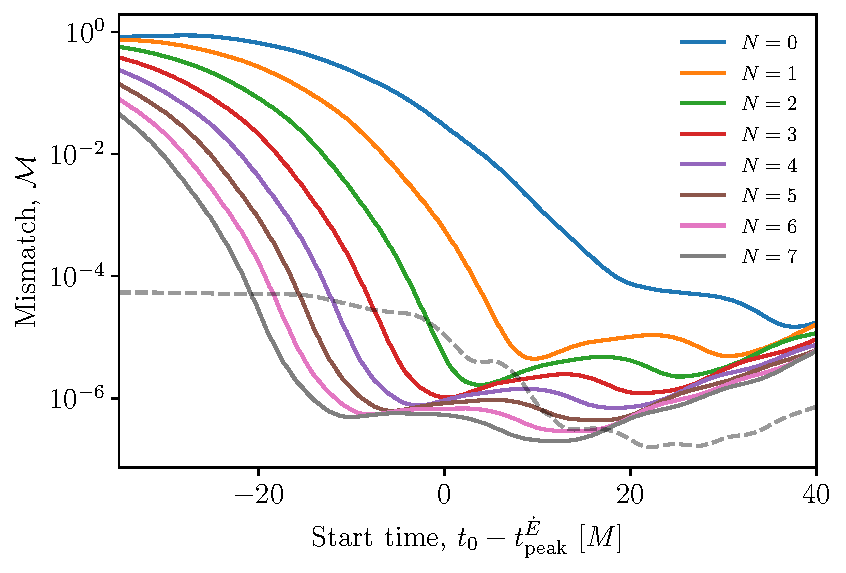
\includegraphics[width=0.6\columnwidth]{ModellingTheRingdownFromPrecessingBlackHoleBinaries/1856_mismatch_vs_t0_mirror_modes_with_error_edit.pdf}
    \caption[Mismatch for the mirror-mode model fitted to SXS:BBH:1856]{
    Mismatch as a function of ringdown start time for the mirror-mode model (Eq.~\ref{ch2:eq:mirror_model}) when fitting to the rotated $h'_{22}$ mode of the NR simulation SXS:BBH:1856.
    Comparing with Fig.~\ref{1856_mismatch_vs_t0}, the locations of the mismatch minima are roughly unchanged in time, but the inclusion of mirror modes reduces the mismatch to values similar to those in Fig.~\ref{305_mismatch_vs_t0}. The dashed grey curve shows the estimate of the error in the underlying NR simulation and is described in Section~\ref{NR_error_appendix}.
    }
    \label{1856_mirror_mode_mismatch_vs_t0}
\end{figure}

\begin{figure}[t]
    \centering
    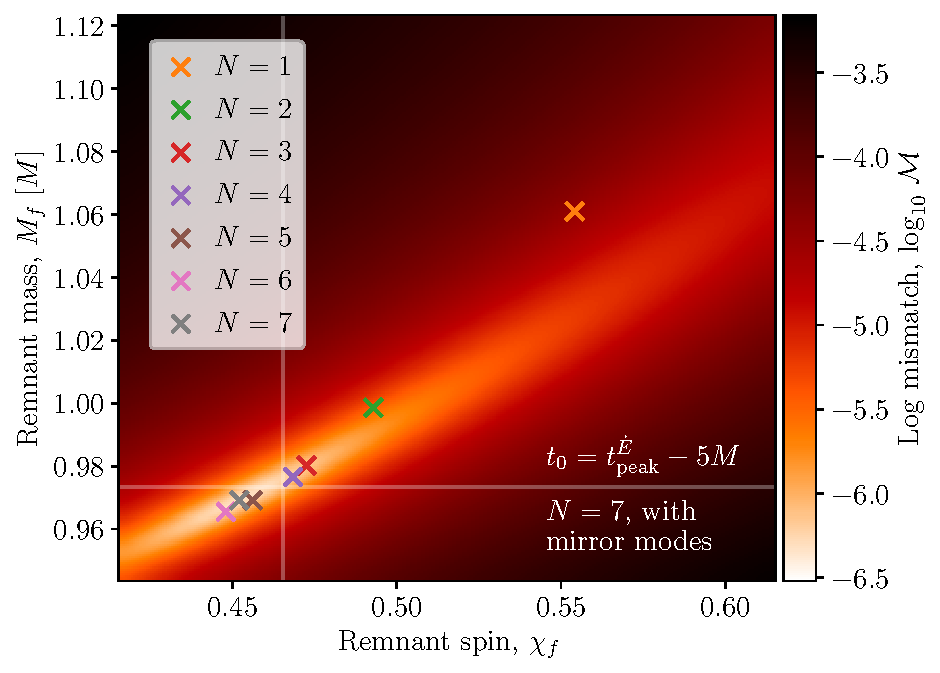
\includegraphics[width=0.6\columnwidth]{ModellingTheRingdownFromPrecessingBlackHoleBinaries/1856_epsilon_grid_mirror_modes_m5.pdf}
    \caption[Recovery of SXS:BBH:1856 remnant properties using the mirror-mode model]{ 
    Recovery of the SXS:BBH:1856 remnant properties when fitting the mirror-mode model (Eq.~\ref{ch2:eq:mirror_model}) to the rotated $h'_{22}$ mode from $5M$ before the time of its peak energy flux.
    The heat map shows the mismatch for the fit with $N=7$, while the crosses show the locations of the minima in the mismatch for fits performed with different values of $N$ ($N=0$ lies outside the figure, and is not included for clarity). 
    Comparing with Fig.~\ref{1856_epsilon_grid}, the inclusion of mirror modes sharpens the mismatch peak and achieves smaller mismatch values. 
    However, when averaged across the population of precessing simulations, the mirror-mode model doesn't give smaller values for the remnant error (see dashed curve in Fig.~\ref{misaligned_spin_epsilon_hist}). 
    Here, $\epsilon = 0.014$ for the $N=7$ model.
    }
    \label{1856_mirror_mode_epsilon_grid}
\end{figure}

To investigate whether the choice of ringdown start time could be contributing to the wider histograms seen in Fig.~\ref{misaligned_spin_epsilon_hist}, the behaviour of the mismatch heat maps (e.g.\ Figs.~\ref{305_epsilon_grid}, \ref{1856_epsilon_grid}, \ref{1856_mirror_mode_epsilon_grid}) with varying start time was explored for selected SXS simulations. 
Animations of ringdown fits with varying start time can be found at Ref.~\cite{finch_eliot_2021_4538194}.
For the aligned-spin simulation SXS:BBH:0305, we see that the location of the mismatch minimum in the mass-spin plane settles on the true remnant properties for a sufficiently late choice of the start time ($t_0 \geq t_{\mathrm{peak}}^{h_{22}}$ for the $N=7$ overtone model). 
In addition, the mismatch minimum stays centred on the true remnant properties until numerical noise takes over.
For earlier choices of the start time, the $N=7$ overtone model gives biased values for the final mass and spin, see Ref.~\cite{finch_eliot_2021_4538194}.
Applying the $N=7$ overtone model to the misaligned-spin simulation SXS:BBH:1856, we see that the location of the mismatch minimum moves around the mass-spin plane as start time is varied. Even at late times, it never settles on the true remnant properties.
The inclusion of mirror modes, as seen in Fig.~\ref{1856_mirror_mode_epsilon_grid}, narrows the mismatch minimum. The movement of the mismatch minimum around the mass-spin plane is reduced as well, however it still doesn't settle on the location of the true remnant properties.
This behaviour may explain some of the observed widening of the histograms, and perhaps hints something is missing from the ringdown model.


\subsection{Higher harmonics}\label{kitchen-sink}

As demonstrated by Fig.~\ref{misaligned_spin_epsilon_hist}, %(and also Fig.~\ref{misaligned_spin_epsilon_hist_m10} in appendix \ref{appendix_a})
the overtone and mirror-mode models considered so far achieve median values for the remnant error $\epsilon \sim 0.01$, a factor of 10 or more higher than the aligned-spin fits of Fig.~\ref{aligned_spin_epsilon_hist}. In addition, the spread of $\epsilon$ values recovered is significantly larger, leading to values of $\epsilon$ up to $\sim 0.1$. 
These models perform significantly worse in some cases for precessing systems than aligned-spin systems.

We now investigate whether the inclusion of higher harmonics (that is, QNMs with $\ell > 2$) can improve the fits to $h'_{22}(t)$.
These higher harmonics were neglected by both the overtone (Eq.~\ref{GieslerRD}) and mirror-mode (Eq.~\ref{ch2:eq:mirror_model}) models.
However, mode mixing does occur as a consequence of the different angular basis functions used in the waveform decompositions in Eqs.~\ref{ch2:eq:spherical_expansion} and \ref{ch2:eq:spheroidal_expansion} and the fact that these basis functions are not mutually orthogonal~\cite{Berti:2014fga}.
The amount of mode mixing between the spherical mode ${}_{-2}Y_{\ell m}$ and the spheroidal mode ${}_{-2}S_{\ell m n}$ is determined by the remnant spin $\chi_f$ and the QNM frequency. This can be quantified by how much these functions fail to be orthogonal; i.e.\ by the spherical-spheroidal mixing coefficients (Eq.~\ref{ch2:eq:mu}).
A translational offset between the NR and ringdown frames (e.g.\ due to a kick) can also lead to mixing between $m$-modes~\cite{Boyle:2015nqa}; this effect is neglected here.
To include the contribution from higher harmonics, we define a new ringdown model for the spherical-harmonic modes which now allows for a sum over different $\ell$:
\begin{equation}\label{full_ringdown}
    h_{\ell m}^{N,\,L,\, {\rm mirror}}(t) = \sum_{n=0}^N \sum_{l=2}^{L} \qty[ C_{l m n} e^{-i \omega_{l m n}(t-t_0)} + C'_{l m n} e^{i \omega^*_{l m n}(t-t_0)} ]\quad \textrm{for} \quad t \geq t_0.
\end{equation}
This \emph{harmonic} model contains all of the allowed QNMs in Eq.~\ref{ch2:eq:spheroidal_expansion}, including the mirror modes and the overtones.
This comes at the expense of a large number of free parameters; there are $4(N+1)(L-\ell+1)$ in the complex amplitudes, plus the two remnant parameters $M_f,\; \chi_f$ that determine the complex QNM frequencies.

\begin{figure}[t]
    \centering
    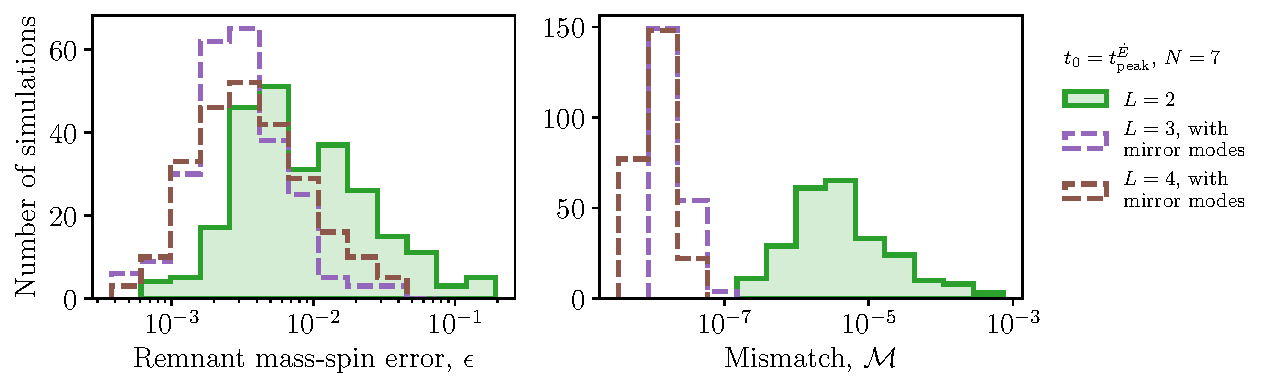
\includegraphics[width=\columnwidth]{ModellingTheRingdownFromPrecessingBlackHoleBinaries/misaligned_spin_epsilon_M_hist_harmonics.pdf}
    \caption[Remnant-property errors and mismatches for the harmonic model fitted to misaligned-spin SXS simulations]{
    \emph{Left:} histograms of the mass-spin remnant error $\epsilon$ from harmonic model fits (Eq.~\ref{full_ringdown}) to the same 252 misaligned-spin SXS simulations used in Fig.\ref{misaligned_spin_epsilon_hist}. 
    Shown (in dashed lines) are the $N=7$, $L=3$ and $L=4$ models with mirror modes. 
    Also shown in green is the overtone model with $N=7$ and $L=2$ (no mirror modes); this is the same as the green histogram in Fig.~\ref{misaligned_spin_epsilon_hist} and is included here to aid comparison. 
    \emph{Right:} histograms of the mismatch from a fit with the true remnant mass and spin parameters, with the same models and SXS simulations as in the left histogram. 
    The harmonic model, which includes many free parameters, achieves small mismatches but without significant improvement in the remnant error. 
    We note that the inclusion of $L=4$ does not bring any additional improvements over $L=3$.
    }
    \label{misaligned_spin_epsilon_hist_harmonics}
\end{figure}

Multiple variations of this harmonic model were trialled (varying $N$, $L$, and the inclusion of mirror modes) on the same population of 252 misaligned-spin SXS simulations.
Fig.~\ref{misaligned_spin_epsilon_hist_harmonics} shows the chosen subset of results, which includes the $N=7$, $L=3$ and $L=4$ models (both with mirror modes). As before, we fit to the rotated $h'_{22}(t)$ spherical harmonic mode.
To make a clear comparison with the previous models, we again use a ringdown start time corresponding to the peak of the GW energy flux.

The inclusion of higher harmonics (dashed histograms in Fig.~\ref{misaligned_spin_epsilon_hist_harmonics}) drastically improves the mismatch.
A small mismatch is not surprising for a model with so many free parameters, and in some of these cases we are likely pushing beyond the limits of accuracy of the NR simulations. See Section~\ref{NR_error_appendix} for a discussion of the numerical errors.
There is a modest reduction in $\epsilon$ for some systems, and in particular we see less systems with $\epsilon > 0.01$ (at least for $L=3$). This hints at the importance of higher harmonics in some precessing systems. Despite this, we still see worst-case values of $\epsilon \sim 0.04$.


\section{Surrogates}\label{surrogate-section}

NR simulations are computationally expensive, and although the number of simulations available in public catalogs is growing they are still limited in their parameter space coverage. 
NR surrogate models~\cite{Blackman:2015pia, Blackman:2017pcm, Varma:2019csw, Varma:2018mmi} would appear to be an attractive alternative.
These models use reduced-order and surrogate modelling techniques to extend the results of a set of NR simulations smoothly across parameter space. 
The use of surrogates could, in principle, allow us to extend the results of this chapter to include many more systems as well as allowing us to study how the excitations of the various QNMs vary during a smooth exploration of parameter space.
However, care must be taken as the surrogate modelling necessarily introduces an additional source of error into the waveforms, on top of the errors originally in the NR waveforms themselves.
 
When attempting to fit QNM ringdown models with overtones to NRSur7dq4~\cite{Varma:2019csw} waveforms, it was found that incorrect values for $M_f$ and $\chi_f$ were being recovered (particularly at high mass ratios). This being the case even for aligned-spin or non-spinning systems. Although the NRSur7dq4 waveforms do not provide the remnant properties, these can be obtained via NRSur7dq4Remnant~\cite{Varma:2019csw} (it was found the problem did not lie with the values returned by NRSur7dq4Remnant but rather with the waveform surrogate).

\begin{figure}[t]
    \centering
    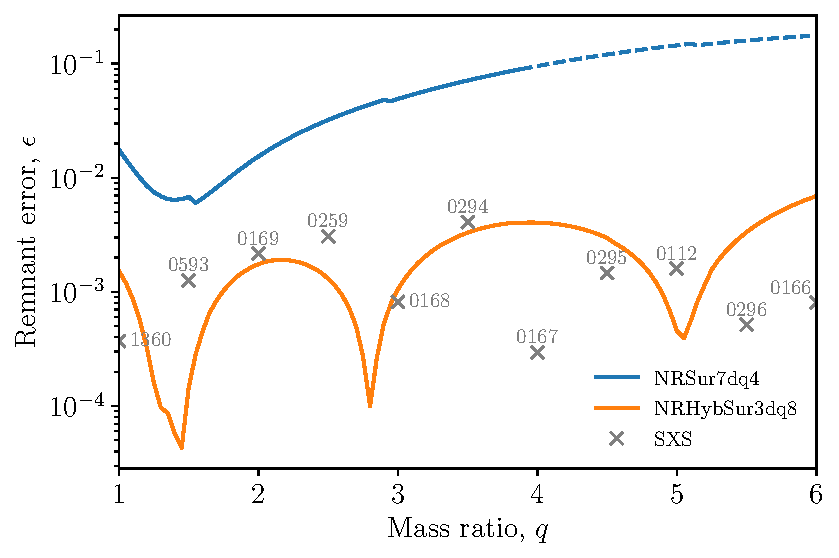
\includegraphics[width=0.6\columnwidth]{ModellingTheRingdownFromPrecessingBlackHoleBinaries/surrogate_epsilon_and_mass_ratio.pdf}
    \caption[Comparison of remnant-property errors from two surrogate models and a selection of SXS simulations]{
    Comparison of the remnant error $\epsilon$ from two surrogate models and a selection of SXS simulations. All are zero initial spin. The fits were performed on the $h_{22}$ mode with the $N=7$ overtone model, Eq.~\ref{GieslerRD}, starting from the time of peak strain. The labels on each cross correspond to the SXS ID. The dashed line indicates where we are outside the training range of NRSur7dq4.
    }
    \label{surrogate_epsilon_vs_q}
\end{figure} 

To investigate the performance of NRSur7dq4 ringdown waveforms, a series of simulations with zero initial spin with increasing mass ratio $q$ from 1 to 6 were used. 
The $N=7$ overtone model (Eq.~\ref{GieslerRD}) was fitted to the $h_{22}(t)$ mode of each starting from the peak strain (as in Section~\ref{aligned-spin-section})
and the remnant error $\epsilon$ (Eq.~\ref{eq:epsilon}) was calculated for each.
The results are shown in Fig.~\ref{surrogate_epsilon_vs_q}, along with the results for similar fits performed directly on 11 zero-spin SXS simulations at discrete values of the mass ratio. 
The fits to the NRSur7dq4 surrogate produce values for $\epsilon$ that are 1-2 orders of magnitude higher than for the equivalent SXS simulations. 
Also shown are the results from a similar analysis with the more restrictive aligned-spin surrogate NRHybSur3dq8~\cite{Varma:2018mmi, Varma:2018aht}; this was found to be in close agreement with the SXS simulations.

Residuals and mismatches can also be computed between surrogate and NR waveforms (taking care to align the waveforms in both time and phase).
For SXS:BBH:0168, the $q=3$, zero-spin simulation used in Fig.~\ref{surrogate_epsilon_vs_q}, we find $\sim 2\%$ residuals in the ringdown when comparing to the NRSur7dq4 surrogate with the same parameters. 
This leads to a mismatch between the surrogate and SXS:BBH:0168 of $3.7 \times 10^{-4}$, when integrating over the ringdown. For comparison, we have a $\sim 10^{-6}$ mismatch between the ringdown model Eq.~\eqref{GieslerRD} and the SXS simulation. The relatively high mismatch between the NRSur7dq4 and SXS waveforms translates to the relatively high values of $\epsilon$ seen in Fig.~\ref{surrogate_epsilon_vs_q}. 

It seems that the high-dimensional precessing surrogate NRsur7dq4 is not yet sufficiently accurate in the ringdown for the purposes of QNM overtone studies that, by virtue of their large number of free parameters, fit the ringdown with very small mismatches. 
By contrast, the lower-dimensional aligned-spin surrogate NRHybSur3dq8 does appear to be sufficiently accurate for such studies.


\section{Numerical relativity errors}\label{NR_error_appendix}

It is important to remember the finite accuracy of the NR simulations used in ringdown studies.
This is particularly true when using models with many QNMs which, by their very nature, use a large number of free parameters and regularly achieve very small ($\sim 10^{-6}$) mismatches.
If care is not taken, we risk fitting our models to the numerical noise. 
In this section we describe the numerical checks performed on the two individual simulations used in this chapter: SXS:BBH:0305, and SXS:BBH:1856. %, and the three simulations shown in Fig.~\ref{misaligned_spin_variation}.
In each case the numerical errors were estimated by comparing results obtained using data from the two highest resolutions (levels) available in the SXS catalog. 

First, we quantify the numerical error in the mismatch.
This was done by calculating the mismatch between the two highest NR resolutions from a time $t_0$ to a time $T = t_0 + 100M$, for a range of $t_0$. For each start time, we optimally align the two waveforms in time (taking the absolute value in the mismatch automatically optimises the mismatch over phase). The alignment in time can be done by matching the time of peak strain, for example, or by numerically rolling the waveform to find the optimal time shift for each mismatch calculation.
The results are shown by the grey dashed lines in the mismatch vs start time plots in Figs.~\ref{305_mismatch_vs_t0}, \ref{1856_mismatch_vs_t0} (duplicated in Fig.~\ref{1856_mirror_mode_mismatch_vs_t0}). % and the 3 panels of Fig.~\ref{misaligned_spin_variation}.
Generally, we see numerical error estimates at or below the model mismatches, particularly at late times, indicating that we are not fitting to the numerical noise.
The main exception is Fig.~\ref{1856_mirror_mode_mismatch_vs_t0} where the mirror-mode model is applied to a precessing system. This is expected; precessing NR simulations, and those with high mass ratios are generally expected to have larger numerical errors. Additionally, the mirror mode and harmonic models have the highest numbers of free parameters making them more likely to reach the accuracy of the NR simulation. 

Second, we investigate the numerical error on the remnant mass and spin.
We quantify the numerical error with $\epsilon_{\mathrm{NR}}$, the Euclidean distance (Eq.~\ref{eq:epsilon}) between the remnant properties reported in the two highest resolution levels of the NR simulation.
The $\epsilon_{\mathrm{NR}}$ values are reported in the previous sections. % and in the table in appendix \ref{appendix_a}.
In all cases $\epsilon_{\mathrm{NR}} < \epsilon$. 
This supports the conclusions in this chapter and indicates they are likely to be robust against numerical noise in the underlying NR simulations used.


\section{Conclusions} \label{sec:discussion}

This chapter has made a first systematic attempt at using QNMs to model the ringdown of BHs formed from BBHs with misaligned component spins in the inspiral.
Previously, for aligned-spin systems, it has been found that the ringdown can be modelled with low mismatch and low remnant errors using a model that includes overtones of the fundamental QNM~\cite{Giesler:2019uxc}. 
For seven overtones, the ringdown can be reliably modelled from the peak of the $h_{22}(t)$ strain for a range of SXS simulations.
Additionally, the inclusion of mirror modes can allow the ringdown to be modelled from even earlier times~\cite{Dhani:2020nik}.
In this chapter, which generalised these studies to precessing systems, we find that while QNM models can reliably achieve small mismatches, in the worst cases the remnant errors are more than a factor of 10 higher.
This is the case even when choosing to start the ringdown at the more conservative (i.e.\ later) peak in GW energy flux. 
The inclusion of higher harmonics reduces the remnant error in some cases, perhaps a sign that mode mixing in the ringdown is generally more important in precessing systems. However, in other cases, a bias remains in the recovered remnant properties.
We conclude that it is not possible to reliably model the ringdown from the peak in the flux, or indeed from the peak in the strain. 

We end by sounding a brief note of caution to any who attempt to construct a QNM model starting at or before the peak flux or strain. 
While such a model will work in some cases, it risks biased results in others. 
This risk is subtle because QNM models can give small mismatches even when they fail to adequately describe the remnant.


% \section{Overtone Model Fits to a Variety of Precessing NR Simulations}\label{appendix_a}

% \begin{figure}[h]
%     \centering
%     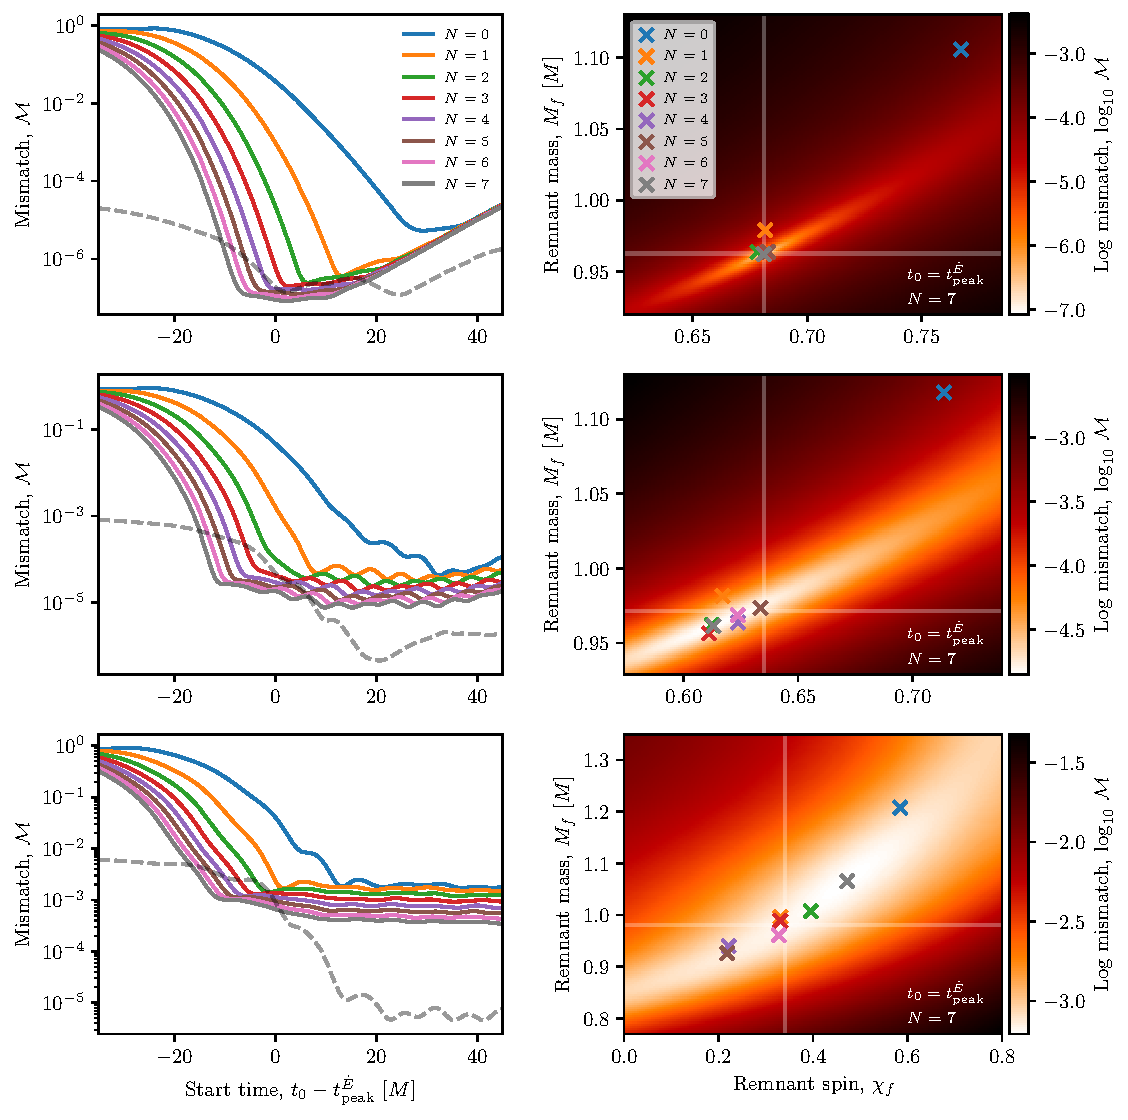
\includegraphics[width=\textwidth]{ModellingTheRingdownFromPrecessingBlackHoleBinaries/appendix_plot_with_error_edit.pdf}
%     \caption[Selection of results for modelling the ringdown of misaligned-spin SXS simulations using the overtone model]{ 
%     A selection of results for modelling the ringdown of precessing NR simulations from the SXS catalog \cite{Boyle:2019kee, Mroue:2013xna,sxs_catalog} using the overtone model in Eq.~\ref{GieslerRD}.
%     These plots show the results for the three systems described in the table that have been chosen to illustrate the wider range of behaviours that occur for precessing systems, from good at the top to bad at the bottom.
%     The left-hand column of plots also shows the difficulty in identifying a general start time for the ringdown as mismatch is minimised for a range of different times and sometimes there isn't even a clear first minimum.
%     }
% 	\label{misaligned_spin_variation}
% \end{figure}

% \begin{footnotesize}
% \begin{center}
% \begin{tabular}{ c|c|c|c|c|c } 
% %\hline
% $\;$SXS:BBH ID $\;$ & $\;$Figure row$\;$ & $\;$Remnant error $\epsilon$$\;$ ($\epsilon_{\mathrm{NR}}$) &  $\;$Mass ratio $q$$\;$ & Component spins $\vb*{\chi}_1$, $\vb*{\chi}_2$  & $\;$Remnant spin $\vb*{\chi}_f$$\;$ \\
% \hline
% 1677 & top & $8.1 \cross 10^{-4}$ ($1.8 \cross 10^{-4}$) & 2.64 & $(-0.06,\,0,\,0.27)$, $(-0.49,\,-0.55,\,0.06)$ & $(-0.05,\,0,\,0.68)$ \\ 
% %\hline
% 1768 & middle & $2.6 \cross 10^{-2}$ ($8.0 \cross 10^{-4}$) & 3.49 & $(0.65,\,0.03,\,0.01)$, $(-0.3,\,0.05,\,0.47)$ & $(0.31,\,-0.02,\,0.56)$ \\ 
% %\hline
% 1789 & bottom & $1.6 \cross 10^{-1}$ ($4.8 \cross 10^{-4}$) & 3.72 & $(0.46,\,0.08,\,-0.52)$, $(-0.43,\,-0.28,\,-0.17)$ & $(0.14,\,0.01,\,0.31)$ \\ 
% %\hline
% \end{tabular}
% \end{center}
% \end{footnotesize}


% \section{Overtone Model Fits to a Population of Precessing NR Systems Starting Before the Peak Flux}\label{misaligned_spin_fits_appendix}

% The analysis on the population of misaligned-spin simulations performed in section \ref{misaligned-spin-section} (results plotted in Fig.~\ref{misaligned_spin_epsilon_hist}) is repeated here using an earlier start time for the ringdown: $t_0=t^{\dot{E}}_{\rm peak}-10M$.
% This was done to check whether a poor choice of start time was responsible for some of the poor fits obtained using the overtone model in Eq.~\ref{GieslerRD}.
% The new results are plotted in Fig.~\ref{misaligned_spin_epsilon_hist_m10}.
% We find that the $N=7$ model results do not significantly change with the new start time.
% The $N=3$ and $N=0$ model results do change and generally give a worse fit with the earlier start time, as might be expected. This analysis shows that the overtone model (with or without mirror modes) cannot be reliably applied to precessing systems at early times. 

% \begin{figure*}[h]
%     \centering
%     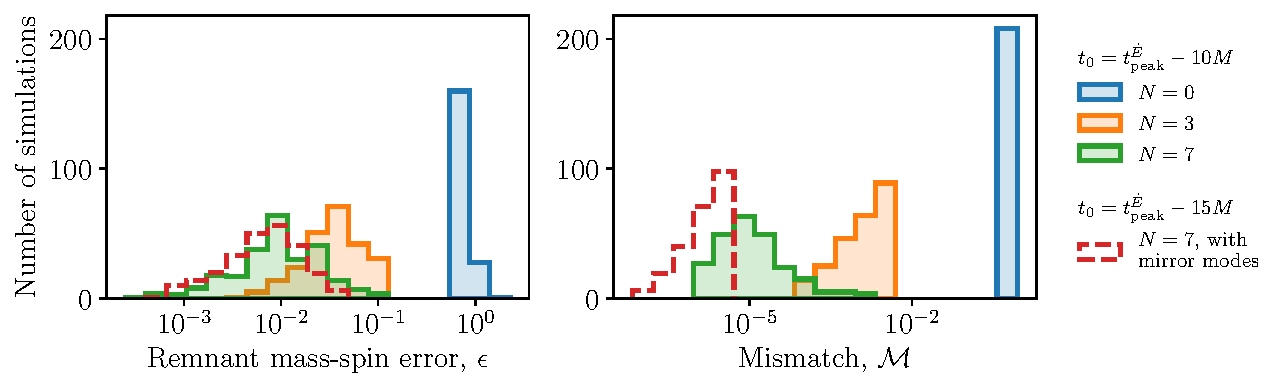
\includegraphics[width=\columnwidth]{ModellingTheRingdownFromPrecessingBlackHoleBinaries/misaligned_spin_epsilon_M_hist_m10.pdf}
%     \caption[Remnant error and mismatches for fits to misaligned-spin SXS simulations using the overtone model starting from $10M$ before the peak of the $h_{22}$ strain]{
%     Left: histograms of the mass-spin remnant error $\epsilon$ from an overtone model fit to the rotated $h'_{22}$ mode of 252 misaligned-spin SXS simulations for several different overtone numbers $N$. 
%     Right: histograms of the mismatch from a fit with the true remnant mass and spin parameters, with the same overtone models and SXS simulations as in the left histogram.
%     %
%     These results are similar to those in Fig.~\ref{misaligned_spin_epsilon_hist} in the main text, but use a start time that is earlier by $10M$.
%     %
%     The solid histograms show results from fits performed starting $10M$ before the peak of the energy flux with $N$ overtones of the fundamental $\ell = m = 2$ mode.
%     The red dashed line shows results from a $N=7$ model that also includes mirror modes and was fitted with a ringdown starting $15M$ before the peak in the energy flux.
%     }
%     \label{misaligned_spin_epsilon_hist_m10}
% \end{figure*} 
